\documentclass{article}

% \usepackage{icml2023}
\usepackage[accepted]{icml2023}

% Packages
\usepackage{hyperref}
\usepackage{graphicx}
\usepackage{booktabs}
\usepackage{multirow}
\usepackage{amsmath}
\usepackage{xcolor}
\usepackage{subcaption}

% Aliases
\newcommand{\github}{\href{https://github.com/mikasenghaas/swarm}{GitHub}}
\newcommand{\wandb}{\href{https://wandb.ai/mikasenghaas/swarm}{Weights \& Biases}}
\newcommand{\gist}{\href{https://gist.github.com/mikasenghaas/5fa1aa77ea69f187f531a5889983c249}{GitHub Gist}}

% Colours
\definecolor{bblue}{HTML}{5884E2}
\definecolor{oorange}{HTML}{F19E38}

% Running Title
\icmltitlerunning{DiLoCo-SWARM}

\begin{document}

% Title
\twocolumn[
  \icmltitle{DiLoCo-SWARM: Early Steps Towards Scalable Decentral Learning}
  \begin{icmlauthorlist}
    \icmlauthor{Mika Senghaas}{epfl}
  \end{icmlauthorlist}
  \icmlaffiliation{epfl}{EPFL}
  \icmlkeywords{Distributed Training, Decentralized AI, SWARM, DiLoCo}
  \vskip 0.3in
]

% Abstract
\begin{abstract}
  ...
\end{abstract}

\section{Introduction}

% Centralized training
Modern foundation models have billions of parameters and are trained on
trillions of tokens~\cite{kaplan2020,hoffmann2022,brown2023}. Operating at such
scale requires orchestrating thousands of GPUs to distribute
computation~\cite{dubey2024,deepseekai2024}. However, traditional
parallelization techniques rely on fast interconnect to not bottleneck the
training. Hence, frontier-scale models are currently trained in high performance
clusters (HPC). Operating HPCs requires billions of dollars, leaving research
capabilities to a small number of corporate and state
entities~\cite{intellect1}. 

% This creates significant points of control, and in turn increases the risk of
% capability capture or misue.

% Decentralized training
Recently, decentralization has emerged as a promising counter-weight to this
trajectory. Decentralized training aims to pool the vast, cheap compute
resources across the globe for collaborative model training. It promises smaller
actors access to large-scale compute at significantly reduced cost, with the
potential to accelerate open-source AI development.  However, this new paradigm
comes with significant technical and algorithmic challenges: nodes have to
communicate via common internet connections, leading to orders of magnitude
lower network bandwidths, and the pool of training nodes can be heterogeneous -
nodes may have varying performance - and dynamic - nodes may join or leave
training unpredictably.

% Intellect-1 and DiLoCo
Hence, current decentral training efforts can not yet match the scale and
efficiency of the centralized setting. Yet, the field is progressing rapidly and
is gaining interest in the research community. INTELLECT-1~\cite{intellect1} is
the most recent demonstration that large-scale decentral model training is
possible. It is a 10B parameter model trained across three continents. The model
is a scale-up of DiLoCo~\cite{douillard2023}, a low-cost communication
distributed data parallel (DDP) training method. Compared to traditional DDP,
DiLoCo's key insight is to replace regular gradient synchronization at every
step with less frequent synchronization using an dual optimization scheme. Their
empirical results show that the method preserves performance while requiring a
fraction of the communication cost, i.e. only every 500 steps. The experiments
have since been replicated~\cite{jaghouar2024}, and engineered further to enable
billion-parameter training runs in the form of INTELLECT-1~\cite{intellect1}.
However, a key limitation is that each node has to store a full copy of the
model to participate during training, and that heterogeneous compute can
bottlenecks compute utilization. For this reason, the minimum requirement for a
node were 8xH100 GPUs to contribute to training INTELLECT-1.

% SWARM
SWARM~\cite{ryabinin2023} parallelism is a promising, but less explored,
alternative for decentralized training that is designed for larger scale. Unlike
DiLoCo, which relies solely on data parallelism, SWARM combines two types of 
parallelism - data and pipeline paralleparallelism. By also sharding the model,
SWARM can scale to larger models, or vice versa, allow lower-end devices to
participate in training. This makes it an attractive candidate for further
scaling decentralized training efforts. In its original formulation, SWARM
requires gradient synchronization between all nodes serving the same pipeline
stage of a model. 

% DiLoCo-SWARM
The successes and robustness of DiLoCo motivates this research which investigates
whether step-wise gradient synchronization in SWARM pipeline stages can be replaced
by DiLoCo-style synchronization. We make the following two contributions:

\begin{enumerate}
  \item \textbf{DiLoCo-SWARM.} We show that SWARM parallelism is compatible with
  DiLoCo-style gradient synchronization, allowing to train SWARM while requiring
  significantly fewer synchronization of gradients while retaining
  generalization performance.
  \item \textbf{Implementation.} We release a minimal training script
  implementing a feature subset of SWARM parallelism, as well the DiLoCo
  optimizer.  Instead of multiple thousands, the implementation uses a few
  hundred lines of pure PyTorch code.
\end{enumerate}

Besides open-sourcing the full experiment code and results on \github{} and
\wandb{}, we release a distilled version of the training logic as a \gist{}. We
hope that these resources will serve as a starting point for further open-source
research efforts with SWARM, and spark interest in scaling SWARM from research to
production-grade systems, similarly to development of DiLoCo.

\section{Background}

\subsection{Distributed Training}

In distributed training, $n$ nodes collaboratively train a \textit{model}
$f_{\theta}$ parameterized by its weights $\theta$, on a \textit{dataset} of
samples $D = \{(\mathbf{x}_e, \mathbf{y}_1),\dots\}$. Collaboration requires
nodes to periodically communicate intermediate results. We will describe two of
the most widely used forms of parallelization, relevant in the context of
DiLoCo-SWARM.

\begin{figure}[h]
    \centering
    \begin{subfigure}[b]{0.22\textwidth}
        \centering
        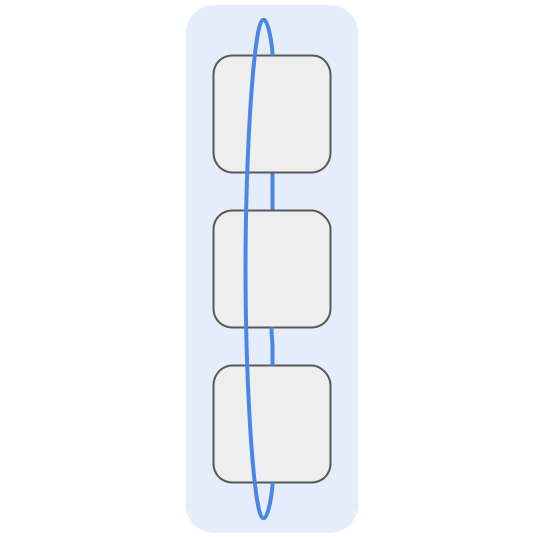
\includegraphics[width=\textwidth]{figures/dp.png}
        \caption{Data Parallelism}
    \end{subfigure}
    \hfill
    \begin{subfigure}[b]{0.22\textwidth}
        \centering
        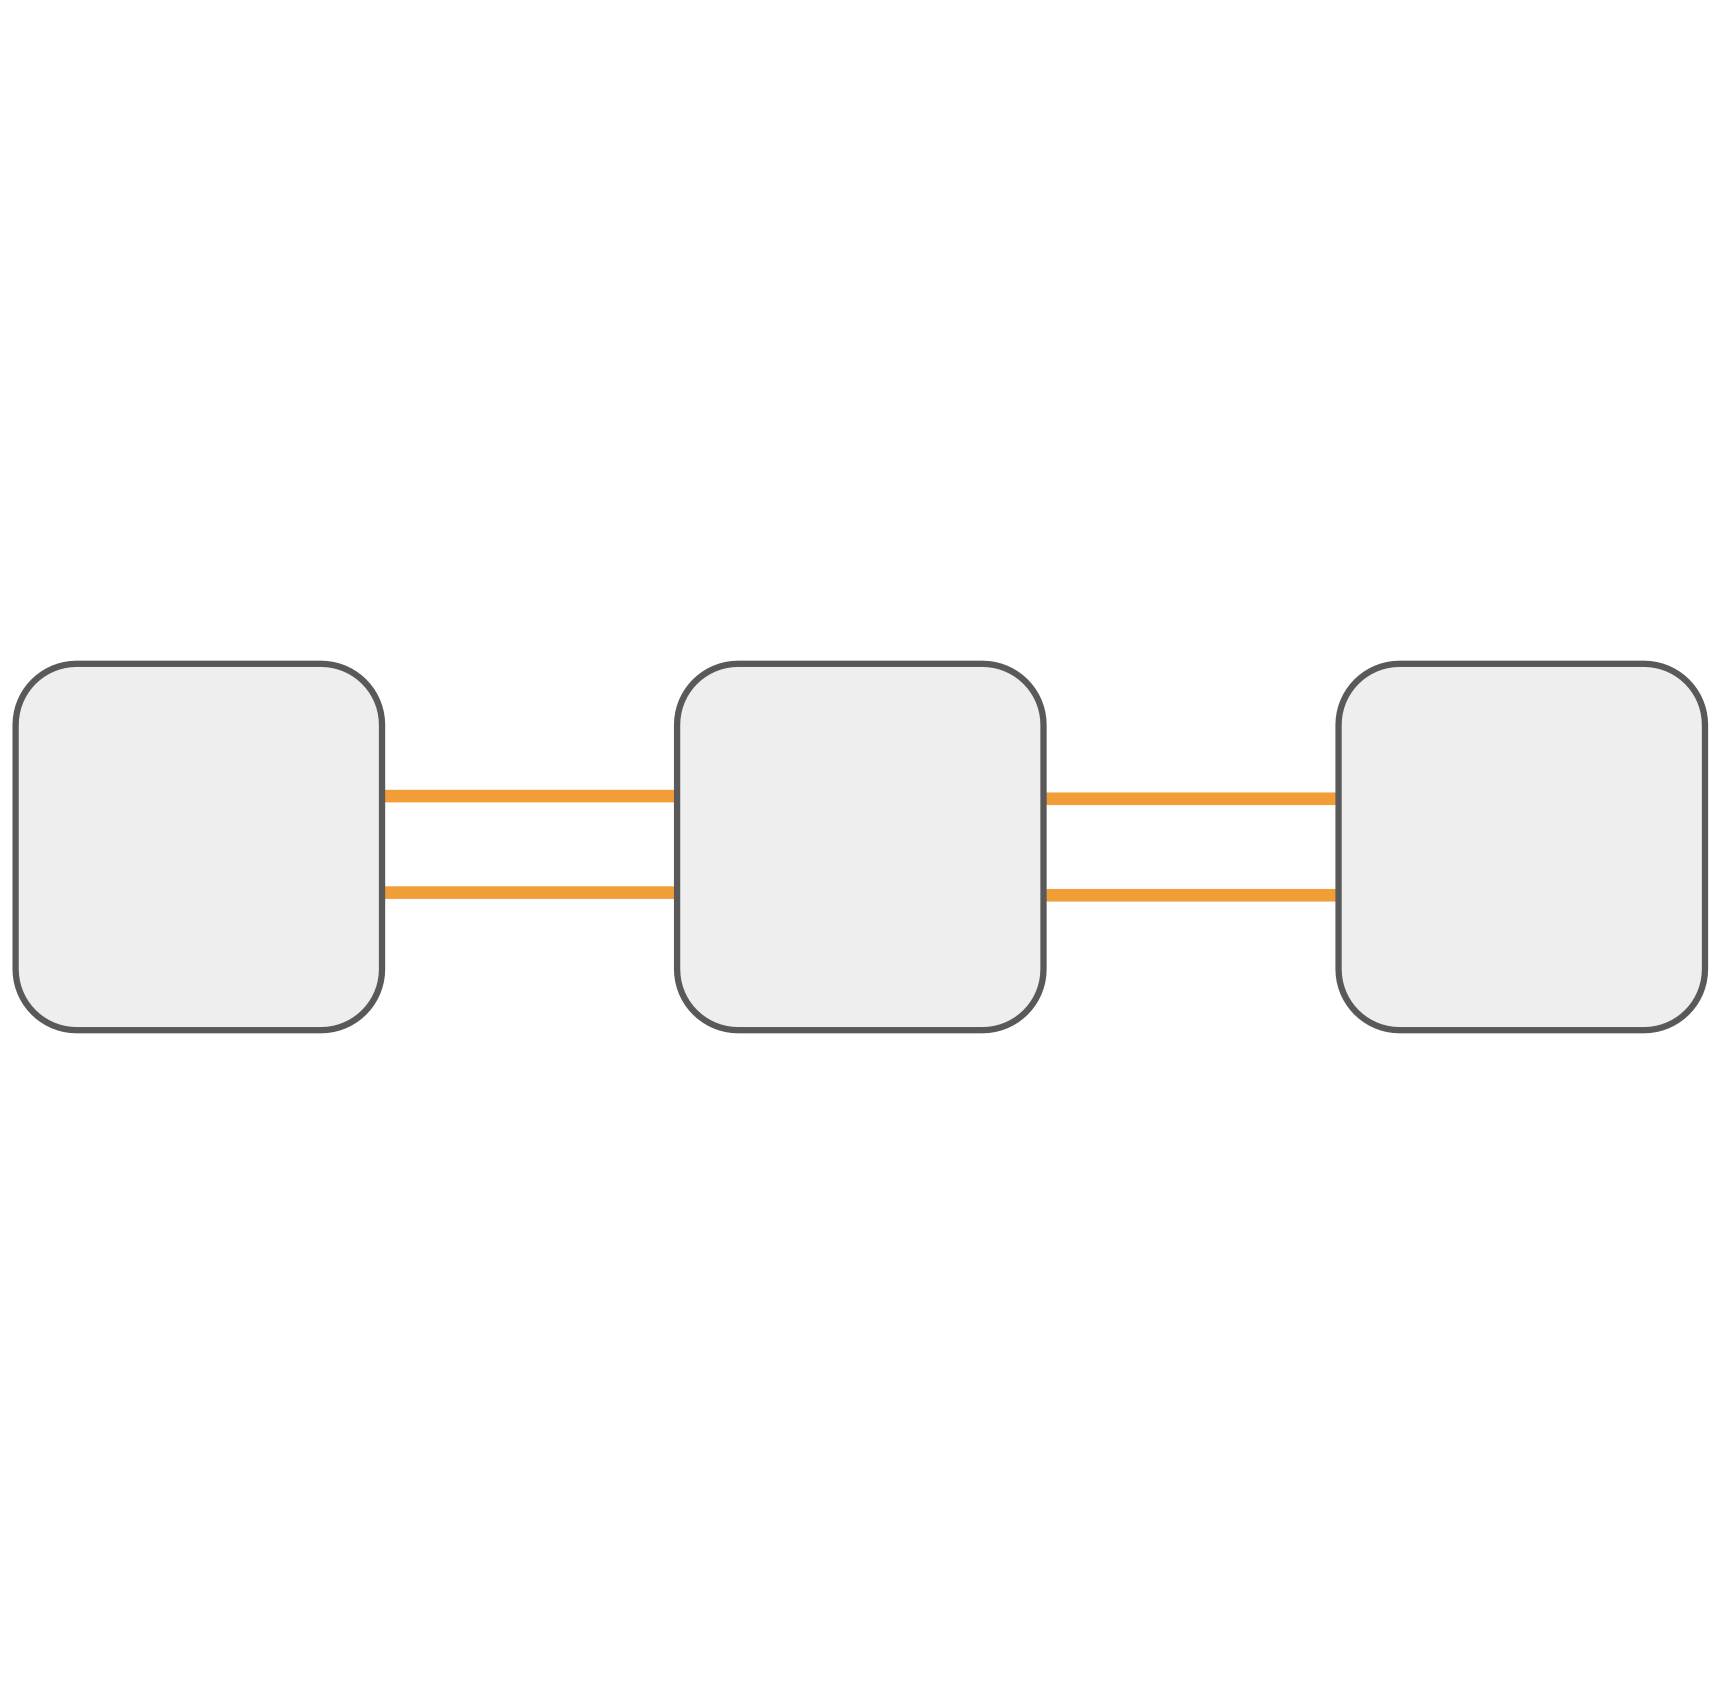
\includegraphics[width=\textwidth]{figures/pp.png}
        \caption{PP Parallelism}
    \end{subfigure}
    \caption{\textbf{DP and PP Communication} High-level visualization of DP and
    PP communication patterns for $n=3$ nodes. Nodes are represented as boxes,
    communication as links. {\color{bblue} Blue links} represent
    \texttt{AllReduce} operations to average gradients between nodes. 
    {\color{oorange}Orange links} represent bi-directional point-to-point
    communication between adjacent stages.}
    \label{fig:dp-pp}
\end{figure}

\textit{Data parallelism} (DP) partitions the dataset, creating $n$ data shards
$D_1,\dots,D_n$. The $i$-th node only holds a (local) data shard $D_i$ and a
copy of the full model parameters $\theta$. Training proceeds as shown in
Algorithm~\ref{alg:dp}: Each node samples a batch from its local data shard,
computes local gradients via a full forward and backward pass, but before
updating the model, averages the gradients from all workers via an
\texttt{AllReduce} operation. DP communication cost scales with the number of
model parameters and number of nodes.

\begin{algorithm}
\caption{Data Parallel Gradient Synchronization}
\label{alg:dp}
\begin{algorithmic}
\STATE {\bfseries Input:} Local Dataset $D_i$, Model $\theta^{(t-1)}$, Optimizer $\mathtt{OPT}$, Loss $\mathcal{L}$
\STATE Sample batch: $x_i\sim D_i$
\STATE Compute gradient: $g_i \gets \nabla_{\theta_i} \mathcal{L}(x_i; \theta^{(t-1)})$
\STATE Sync gradients: $g \gets \frac{1}{n}\sum_{i}^n g_i$ \COMMENT{$\mathtt{AllReduce}$}
\STATE Update model: $\theta_i^{(t)} \gets \mathtt{OPT}(\theta_i^{(t-1)}, g)$
\end{algorithmic}
\end{algorithm}

\textit{Pipeline parallelism} (PP) partitions the model, creating $n$ model
shards $f'$ parameterized by $\theta_1,\dots,\theta_n$, such that the full model
is reconstructed by concatenation of the shards, i.e.
$f_{\theta}=f'_{\theta_1}\circ\dots\circ f'_{\theta_n}$. Due to the sequential
dependency, shards represent "stages" in the pipeline, where the $i$-th stage
serves the model shard $f_{\theta_i}$. For most deep learning model such a
sequential partition is natural, as they are architected as repeated
computational blocks. For example, in Transformer one stage handles one or more
Transformer blocks consisting of attention and feed-forward
layers~\cite{vaswani2017}. The partitioning creates a bi-directional
communication pattern between stages during training, as shown in
Figure~\ref{fig:dp-pp}: During a forward pass activations are communicated from
stage $i$ to $i+1$, and during the backward pass gradients are sent from stage
$i$ to $i-1$. Despite its simplicity, PP is notoriously hard to optimize. Naive
implementations suffer from significant GPU idle time, e.g. when the first node
has to wait for the full pipeline forward and backward pass before being able to
compute gradients. Efficient PP implementations therefore rely on micro-batching
and advanced scheduling techniques to be practically viable. PP communication
scales with the number of stages $n$ and the model's hidden dimension.

Typically, different forms of parallelism can be combined. In the case of DP and
PP, a natural combination is to partition both the dataset and model into
$\{D_i\}_{i\in [m]}$ and $\{\theta_j\}_{j\in [n]}$, respectively. This creates a
$m\times n$ grid structure, where the $(i,j)$-th node handles data shard $D_i$
and model shard $\theta_j$. During training, DP and PP communication is
interleaved: First, nodes send activations and gradients (PP communication)
within each of the $i=1\dots,m$ pipelines to accumulate local gradients. Then,
within each stage $j=1,\dots,n$, the nodes run an \texttt{AllReduce} to average
accumulated gradients for their local shard (DP communication).

\subsection{DiLoCo}

In the decentralized setting, interconnect may be slow and so regular gradient
synchronization as shown in Algorithm~\ref{alg:dp} can bottleneck the training
process, especially when scaling to larger models. Distributed Low-Cost
Communication (DiLoCo)~\cite{douillard2023} is data parallel training method
which reduces the frequency at which gradients are synchronized via a dual
optimization scheme. As shown in Algorithm~\ref{alg:diloco} each node trains for
a fixed number of inner steps using a local optimizer. To synchronize with the
remaining workers, it computes and averages its pseudo-gradient (the difference
between the parameters before and after the inner optimization.) with all nodes
via \texttt{AllReduce} to update a global model using an outer optimizer. 

\begin{algorithm}
\caption{DiLoCo Gradient Synchronization}
\label{alg:diloco}
\begin{algorithmic}[1]
\STATE \textbf{Input:} Local dataset $D_i$, Model $\theta^{(t-1)}$, Optimizers $\mathtt{OPT}_{\text{local}}$ and $\mathtt{OPT}_{\text{global}}$, Loss $\mathcal{L}$, Local Steps $H$ 
\STATE Copy global model: $\theta_i^{(t-1)} \gets \theta^{(t-1)}$
\FOR{$H$ steps}
  \STATE Sample batch: $x \sim D_i$
  \STATE Compute gradient: $g_i \gets \nabla_{\theta_i} \mathcal{L}(x_i; \theta_i^{(t-1)})$
  \STATE Update local model: $\theta_i^{(t-1)} \gets \mathtt{OPT}_{\text{local}}(\theta_i^{(t-1)}, g_i)$
\ENDFOR
\STATE Compute pseudo-gradient: $\Delta_i \gets \theta_i^{(t-1)} - \theta^{(t-1)}$
\STATE Sync pseudo-gradients: $\Delta \gets \frac{1}{n}\sum_i^n \Delta_i$ \COMMENT{$\mathtt{AllReduce}$}
\STATE Update global model: $\theta^{(t)} \gets \mathtt{OPT}_{\text{global}}(\theta^{(t-1)}, \Delta)$
\end{algorithmic}
\end{algorithm}

Empirical results show that DiLoCo drastically reduces the frequency at which
gradients need to be synchronized. Despite only synchronizing every $500$ local
steps, they can match the generalization performance of a DP baseline. However,
DiLoCo shares many challenges with traditional data parallel training. Most
notably, DiLoCo does not scale naturally to models that do not fit into the
local workers' memory - relying on slow parameter offloading
methods~\cite{rhu2016, cui2016}, gradient quantization~\cite{intellect1} and
other tricks for scaling, which come at the cost of reduced efficiency for
scaling, which come at the cost of reduced efficiency

\subsection{SWARM}

PP presents itself as a natural solution. However, in its original formulation 
it does handle heterogeneous and dynamic node setups well, as often found in
decentralized settings. Due to its inherently sequential nature, the pipeline
is bottlenecked by its weakest link, leading to idle time for quicker workers.
Furthermore, a single node failure will stall the entire training procedure,
rendering the algorithm not fault-tolerant.

SWARM parallelism~\cite{ryabinin2023} proposes a decentralized training
framework combining DP and PP. Instead of organizing nodes in a rigid
two-dimensional grid, SWARM constructs stochastic pipelines on-the-fly, as shown
in Figure~\ref{fig:swarm}. First, activations are forwarded stochastically based
on statistical estimates on the throughput of adjacent peers. This ensures that
faster or better-connected nodes receive more requests and sit less idle in
heterogeneous compute settings. Once all micro batches within a step are
processed, local gradients of models shards are averaged within pipeline stages
via an \texttt{AllReduce}. Further mechanisms ensure the algorithm's resilience
to faults: For examle, forward or backward requests which are not fulfilled
after some timeout, are re-routed and the suspected node is temporarily excluded
from training. Further, nodes periodically switch from under- to overutilised
stages to distribute workload.

\begin{figure}[h]
  \centering
  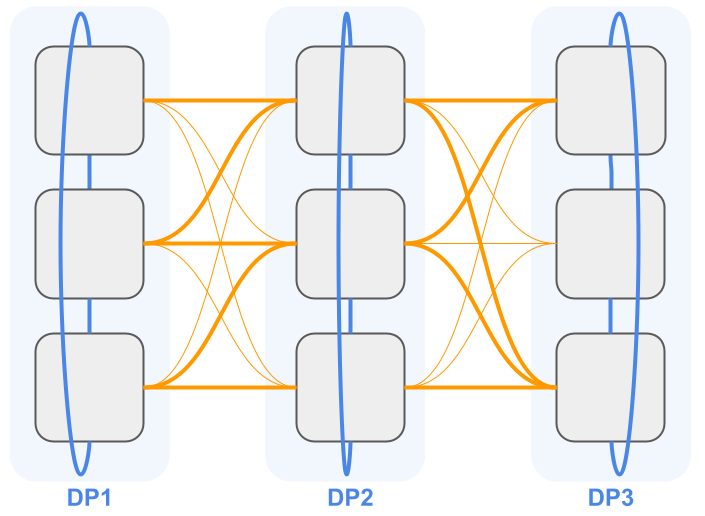
\includegraphics[width=0.45\textwidth]{figures/swarm.png}
  \caption{\textbf{SWARM Communication} We show high-level communication
  patterns in a 3x3 SWARM. SWARM interleaves PP and DP communication: First,
  activations take stochastic forward route through pipeline stages, gradients
  follow the same path backwards such that nodes accumulate gradients. Finally,
  gradients are averaged within stages via \texttt{AllReduce}.}
  \label{fig:swarm}
\end{figure}

% TODO: Add key observation of square-cube law
% -> DP communication scales cubic, PP communication only quadratic

\subsection{DiLoCo-SWARM}

One of two communication types in SWARM relies on costly gradient
synchronization between nodes in pipeline stages at every step. The success and
robustness of DiLoCo in replacing frequent gradient synchronization, motivates 
utilizing DiLoCo-like gradient synchronization, as described in
Algorithm~\ref{alg:diloco} as a drop-in replacement for regular gradient
synchronization within SWARM pipeline stages. We refer to this method as
DiLoCo-SWARM.

\section{Implementation}

A key contribution of this work is the release of a minimal distributed training
script. Depending of its parameterization, it runs a multi-node training job
using data parallelism, tensor parallelism, or a SWARM-style combination of the
two. By optinally specifying an outer optimizer, the script replaces regular
step-wise gradient synchronization with the DiLoCo-style inner-outer
optimization scheme.

% Advantages
The implementation is designed for simplicity and readability. Instead of the
multiple thousand lines of code in the original implementation, it uses only a
few hundreds with the only dependency being PyTorch. This makes it easy for
anybody with some experience in distributed training to grasp the core ideas and
interaction being various traditional parallelization techniques, and 
state-of-the-art methods, like DiLoCo and SWARM. For small-scale testing, it can
emulate training via threads, allowing for debugging and testing without dozens
of GPUs. Because it natively integrates various parallelization techniques, and
interfaces with HuggingFace for models and datasets, it is the ideal starting
point for quickly verifying research ideas and conducting, as showcased in
DiLoCo-SWARM.

% Limitations (Not feature-complete and less efficienty)
However, as of this point, the re-implementation is not feature-complete. Due to
limitations to PyTorch distributed, it does not yet support dynamic world sizes,
over-the-internet connections, and the SWARM's fault tolerance mechanism such as
re-wiring requests. Therefore, the script can only run distributed application
on single node. While this seems to be miss the point of SWARM parallelism, it
still allows for interesting research regarding the core logic of the system. It
should also be noted that the training script does not match the efficiency
reported in the original paper which uses custom distributed communication and
storage primitives, advanced scheduling, and, whenever possible, overlaps
computation asynchronously, resulting in larger hardware utilization.

% TODO: Show in the Appendix which features are supported and which are not

% NanoGPT
The implementation should therefore be seen as a supplemental resource, which
puts emphasize on understandability, and hackability. Our hope is that it might
have a similar effect of NanoGPT, which now serves as an easy-to-hack and verify
testing ground for novel research within the open-source community.

% Implementation details
For more details on the implementation, design decision and some hacks to
circumvent limitations of PyTorch's distributed package, find more details in
the \href{https://github.com/mikasenghaas/swarm}{GitHub} repository.

\section{Experiments}

% Introduction
In this section we report the experiments validating DiLoCo-SWARM. The experiment
mostly follows the setup and hyper-parameters of DiLoCo~\cite{douillard2023}.

% Dataset
We consider a language modeling task on the FineWeb-Edu~\cite{penedo2024}
dataset, a large pre-training dataset consisting of high-quality web pages
filtered for educational content. We choose this dataset over other common
pre-training datasets due to its high token efficiency allowing to match the
original GPT-2~\cite{radford2019} performance on the
HellaSwag~\cite{zellers2019} benchmark when training the same model with 10x
less data~\cite{karpathy2024}.

% Model and 
Unless otherwise stated, we use a randomly initialized GPT-2 small as our base
model with a total of $\sim$180M parameters. Note, that this is slightly larger
than the original GPT-2 model, as we do not share the parameters of the embedding
matrix and language modeling head.

% Hyper-parameters
Training hyper-parameters are identical to those in DiLoCo~\cite{douillard2023}.
The base optimizer is AdamW with a learning rate of $4\cdot 10^{-4}$, and a
weight decay of $0.01$ which is linearly warmed up. When DiLoCo-style gradient
synchronization applies, we use a Nesterov with a learning rate of $0.7$ and a
momentum of $0.9$ as an outer optimizer. A detailed description of the
hyperparameters is provided in Table~\ref{tab:hyperparameters} in the Appendix.

% Evaluation
Our main evaluation metric is the perplexity on a held-out validation set of 10M
randomly sampled tokens. We evaluate throughout training to show the convergence
against the number of training steps.

% Main Experiment: DiLoCo-SWARM
\textbf{Main Experiment.} Our main experiment setup closely follows that of
DiLoCo~\cite{douillard2023}. We train two baselines and a DiLoCo-SWARM. The
\textit{weak baseline} trains for 2,000 steps on one GPU with a batch size of
512 and sequence length of 1024, for a total training budget of 1B tokens. The 
strong baseline is a 4x2 SWARM, i.e. eight workers distributed in two pipeline 
stages. This baseline performs regular all-reduce gradient synchronization at
every step. The higher compute budget is used to scale the batch size to the
number of worker per stage, leading to a total training budget of 4B tokens.
Finally, we train a 4x2 DiLoCo-SWARM which uses the same setup and compute
budget as the strong baseline but performs the outer optimization step only
every 50 steps.

\begin{figure}[ht]
  \centering
  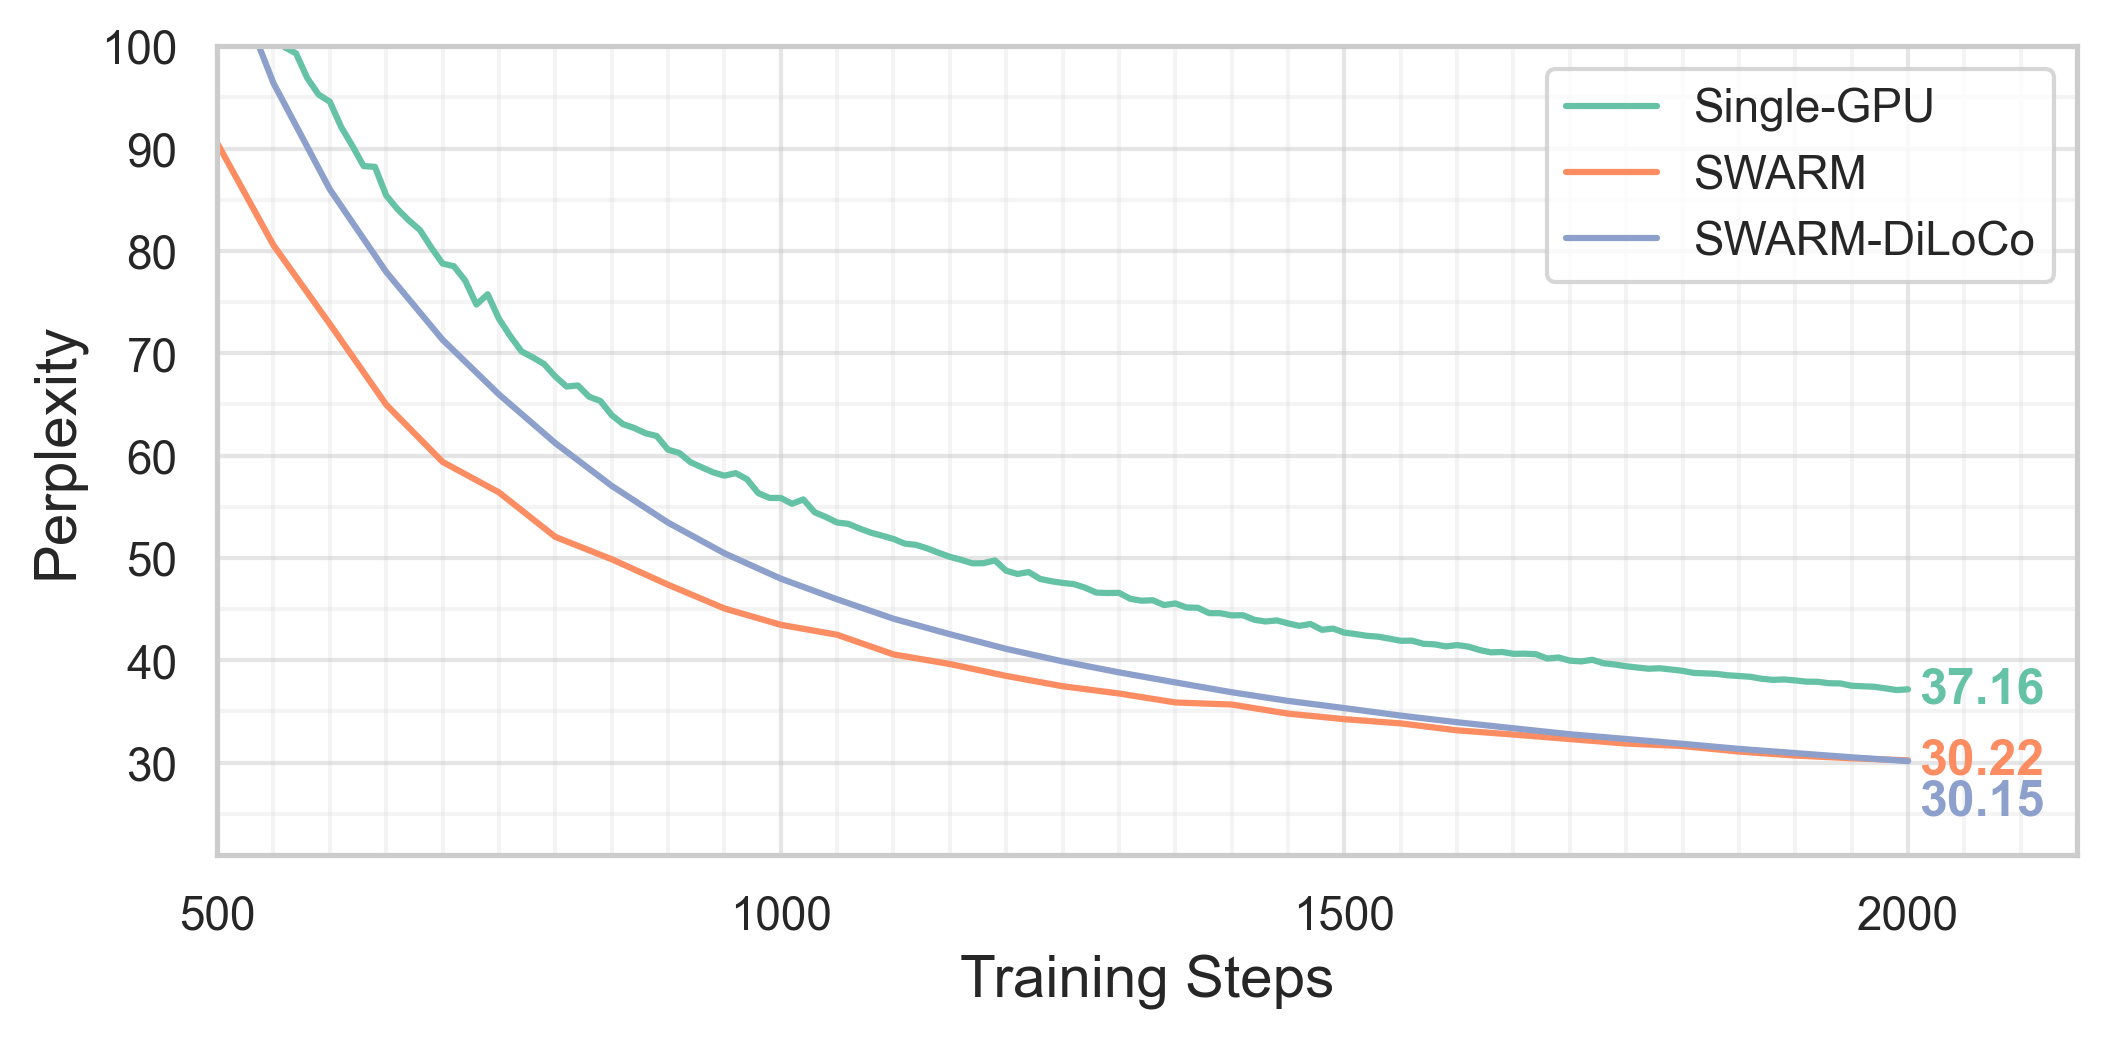
\includegraphics[width=0.45\textwidth]{figures/experiment1.png}
  \caption{\textbf{Main Result} We show the validation perplexity against the number of training steps for two baselines and SWARM-DiLoCo. With the same compute and
  data budget but with 50x less gradient synchronization, DiLoCo-SWARM matches the 
  generalization performance of the strong SWARM baselines.}
  \label{fig:experiment1}
\end{figure}

Figure~\ref{fig:experiment1} shows the validation perplexity as a function of
the training steps. Unsurprisingly, the weaker baseline, using less compute and
data, is outperformed by the stronger SWARM baseline with final perplexities of 
37.16 and 30.22, respectively. Our main finding is that DiLoCo-SWARM closely
matches, and even exceeds, the strong baseline in generalization performance
with a validation perplexity of 30.15, despite synchronizing gradients 50x fewer
times. This implies that DiLoCo-style gradient synchronization is compatible
with SWARM parallelism, allowing to reduce the communication cost incurred by 
gradient synchronization within pipeline stages of SWARM.

% Experiment 2: Ablation on communication frequency
\textbf{Communication Frequency.} We are interested in how \textit{infrequently}
gradient synchronization can occur without impacting convergence. Intuitively,
the slower the frequency, the worse convergence, but whether synchronizing every
10 or 200 steps negatively impacts performance, has implications on the
practical usefulness of the algorithm. To investigate this question we train
five models using the same training setup and only vary the number of local
training steps before performing an outer optimization step.

% TODO: Add perplexities in legend
\begin{figure}[ht]
  \centering
  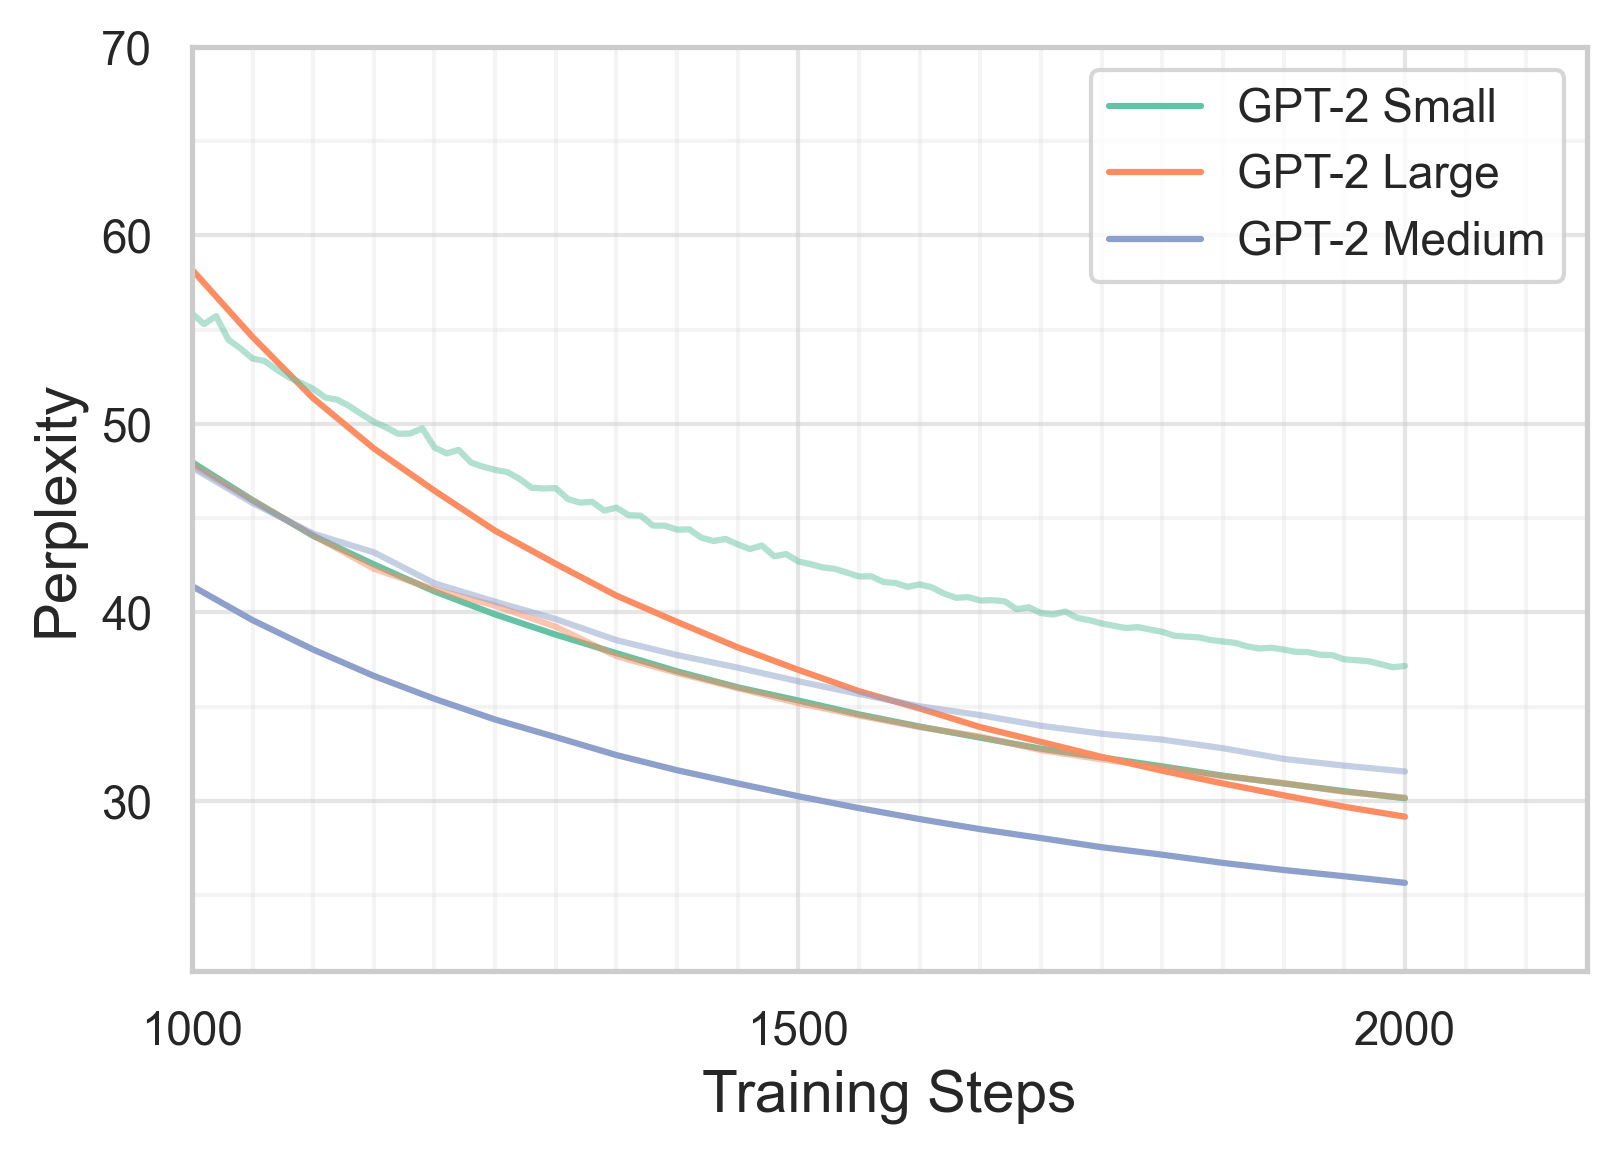
\includegraphics[width=0.45\textwidth]{figures/experiment3.png}
  \caption{\textbf{Communication Frequency} We vary the number of local training
  steps before performing an outer optimization step from $\{10, 20, 50, 100, 200\}$ 
  and report the validation perplexity throughout training. Synchronizing more
  frequently yields better results but performance degradation is neglibible even
  on all tested values.}
  \label{fig:experiment2}
\end{figure}

Figure~\ref{fig:experiment2} shows the results of this experiment. In line with
the original DiLoCo results, generalization performance monotonically increases
with higher gradient synchronization frequency. However, the performance
degradation for less frequent gradient synchronization is mild. As outlined in
Table~\ref{tab:experiment2}, synchronizing every 10 steps achieves a strong
validation perplexity of 27.95. Note, that this also significantly improves the
step-synchronous SWARM baseline in Figure~\ref{fig:experiment1} while still
reducing the synchronization frequency by 10x. In our experiments, a good
trade-off between communication frequency and performance is achieved when
synchronizing every 50 steps, which is therefore used throughout all other
experiments.

\begin{table}[ht]
\centering
\begin{tabular}{lccc}
\toprule
\textbf{Freq.} & \textbf{PPL} & \textbf{$\Delta$ (Abs./Rel.)} \\ 
\midrule
10 & 27.95 & - \\
20 & 28.61 & 0.66 / 2.36\% \\
50 & 30.15 & 2.2 / 7.87\% \\
100 & 30.49 & 2.54 / 9.09\% \\
200 & 31.27 & 3.32 / 11.88\% \\
\bottomrule
\end{tabular}
\caption{\textbf{Communication Frequency} We report the final validation
perplexity for different communication frequencies and their absolute and
relative changes compared to synchronizing every 10 steps.}
\label{tab:experiment2}
\end{table}

% Experiment 3: Varying the model size
Finally, we train different model sizes to check whether the DiLoCo-style
gradient synchronization is robust to model sizes. We use the same setup as the
main experiment but vary the number of layers, heads, and embedding dimensions,
to obtain three different GPT-2 style models. In addition to GPT-2 Small (180M
parameters), we also train GPT-2 Tiny and GPT-2 Medium, with 14M and 405M
parameters respectively.

\begin{table}[ht]
\centering
\begin{tabular}{lccc}
\toprule
\textbf{\# Params} & \textbf{PPL} & \textbf{$\Delta$ (Abs./Rel.)} \\ 
\midrule
180M & 30.15 & 7.01 / 18.86\% \\
400M & 25.66 & 5.91 / 18.72\% \\
800M & & & \\
\bottomrule
\end{tabular}
\caption{\textbf{Model Size} We report the final validation perplexity for
different model sizes and their absolute and relative changes compared to a single GPU baseline.}
\label{tab:experiment3}
\end{table}

Table~\ref{tab:experiment3} shows the the final validation perplexity of the
three models types for the single GPU baseline and the SWARM-DiLoCo setup. We
see that in all instances SWARM-DiLoCO significantly outperforms the weak
baseline by around 18\%, suggesting that DiLoCO gradient synchronization can be
used to synchronize SWARM stages without performance loss independently of the
model shard within the pipeline.

\section{Discussion}

\subsection{Summary}

The findings of this work have implications both for the SWARM and DiLoCo
community. For SWARM, the findings show that DiLoCo-style gradient
synchronization is compatible with SWARM parallelism, allowing to reduce the
communication cost incurred by gradient synchronization within pipeline stages
of SWARM. For DiLoCo, the findings further underline the robustness of the
method, suggesting that DiLoCo-style gradient synchronization is a general
method to reduce communication cost incurred by gradient synchronization. In
addition to the robustness checks in the original work. The experiments provide
evidence to use DiLoCo-style gradient synchronization whenever data parallel
training is used.

\subsection{Limitations \& Future Work}

However, there are many limitations to the current work and loads of future work 
left to be done.

% Experiment environment
Most importantly, all experiments are conducted in a sandbox environment of
reliable and fast interconnect on a single node with eight co-located GPUs.
SWARM was designed for large-scale decentralized training, and so while the 
experiments suggest that DiLoCo-style gradient synchronization is compatible
with SWARM parallelism, it remains to show how the method scales to a realistic
decentralized setting. Hence, an important next step is to integrate the
inner-outer optimization scheme into the original, efficient, SWARM
implementation and conduct experiments on a larger scale. An especially
interesting question is how much of the wall-clock time reduction can be
achieved in more realistic setups.  Within SWARM, there are two types of
communication: inter-stage (pipeline parallel) and intra-stage (data parallel).
While the square-cube law~\cite{ryabinin2023} suggests that gradient
synchronization eventually dominates the communication cost, and the
communication cost is dominated by intra-stage communication, it remains to be
seen how much of the wall-clock time reduction can be achieved in

% Experiment scale (small models, little training steps and data)

% Missing hyperparameter tuning
Another thing to be noted is that this work assumes the DiLoCo hyper-parameters
found in the original work are optimal. While they are likely to be at least
close to optimal, it is an open question whether slightly different hyper-parameters
yield better results.

% How does this behave with different SWARM configurations? (e.g. different
% number of stages and workers?)
Finally, an interesting question is how the method behaves with different SWARM
configurations. SWARM was designed for a large number of workers per stage -
does DiLoCo-style gradient synchronization still yield good results in this
setting?

\section*{Acknowledgements}
\label{sec:acknowledgements}

This work was developed in collaboration with the Scalable Computing Systems
(SaCS) lab at EPFL as well as Prime Intellect. All compute was kindly sponsored
by Prime Intellect.

% Bibliography
\bibliography{references}
\bibliographystyle{icml2023}

% Appendix
\newpage
\appendix
\onecolumn

\section{Appendix}

% Hardware
\textbf{Hardware.} All experiments were conducted on a single node with eight
co-located H100 GPUs on the \href{https://app.primeintellect.com/}{Prime
Intellect Compute} platform.

% Hyperparameters
\textbf{Hyperparameters.} Table~\ref{tab:hyperparameters} shows the
hyperparameters used in the experiments. The outer optimizer parameters is only
used for DiLoCo-style training, else the outer optimization simply synchronizes
the inner model gradients before performing a regular update.

\begin{table}[ht]
\centering
\begin{tabular}{llc}
\toprule
\textbf{Hyperparameter} & \textbf{Value} \\ 
\midrule
\multirow{1}{*}{General} & Batch Size & 512 \\ 
& Sequence Length & 1024 \\ 
& Steps & 2000 \\
\hline
\multirow{1}{*}{InnerOptimizer} & Name & AdamW \\ 
& Weight decay & - \\ 
& Learning Rate & $4 \times 10^{-4}$ \\ 
\hline
\multirow{1}{*}{OuterOptimizer} & Name & Nesterov \\ 
& Learning Rate & 0.7 \\ 
& Momentum & 0.9 \\ 
\bottomrule
\end{tabular}
\caption{Hyperparameters}
\label{tab:hyperparameters}
\end{table}

\end{document}